\section{Motivation}


%The JavaScript engine's performance that involves the compiler,
%garbage collector, etc., and the final display work on GPU are separate issues beyond the scope of this work.

\begin{table}[!t]
\caption{The best-performing available governor}
\vspace{-3mm}
\scriptsize
\begin{center}
        \begin{tabular}{llll}
        \toprule
        &\textbf{Load time}&\textbf{Energy}&\textbf{EDP}\\
        \midrule
            Regular 3G                     &\Performance&\Powersave&\Powersave\\
            \rowcolor{Gray}Regular 4G                     &\Performance&\Conservative&\Interactive\\
            WiFi            &\Interactive&\Ondemand&\Interactive\\
        \bottomrule
        \end{tabular}
\end{center}
\label{tab:best-governor}
\vspace{-5mm}
\end{table}


\begin{figure}[!t]
	\centering
	\subfloat[][Load time]{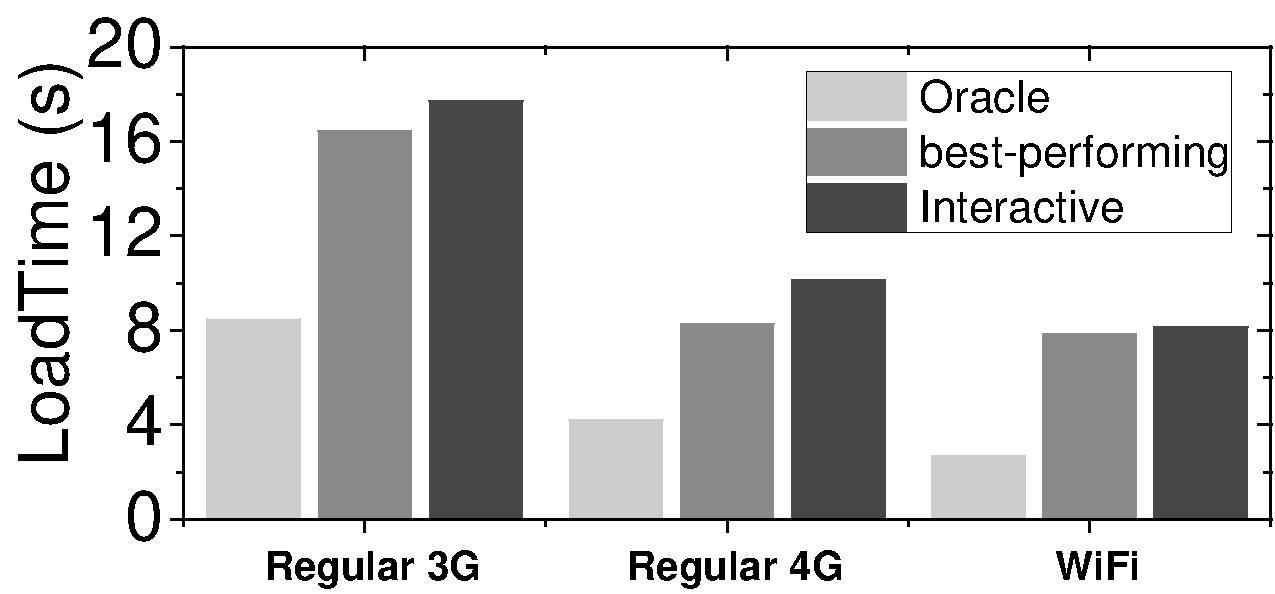
\includegraphics[width=0.22\textwidth]{figure/laod4pagesloadtime.pdf}}
    \hfill
    \subfloat[][Energy consumption]{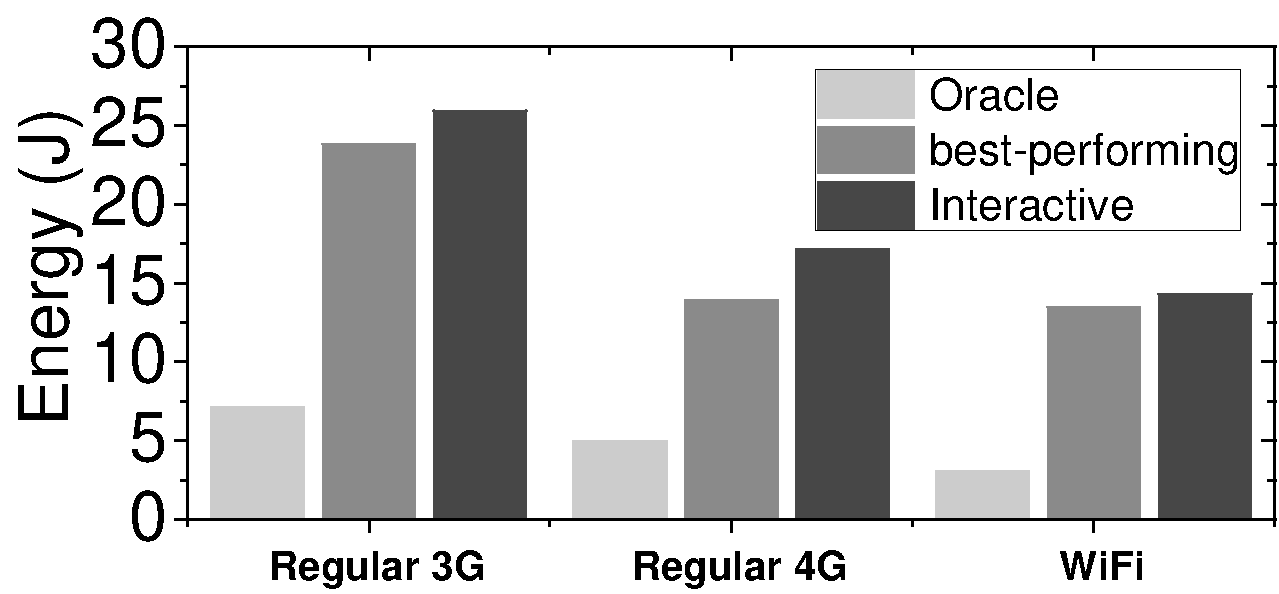
\includegraphics[width=0.22\textwidth]{figure/load4pagesEnergy.pdf}}
    \vspace{-2mm}
    \caption{The achieved total load time (a), energy consumption (b)  when a user was browsing four news pages from \BBCW.
    We show the results for \Oracle, the \bfp existing CPU frequency governor, and \Interactive in three typical networking environments. There is significant room for improvement. }
    \vspace{-5mm}
    \label{fig:motivation}
\end{figure}



Consider a scenario for browsing four \texttt{BBC} news pages, starting from the home page of \BBCW. Our evaluation platform has  a
Cortex-A15 (big) and a Cortex-A7 (little) processors.

\vspace{-1mm}
\cparagraph{Networking Environments.} We consider three typical networking
environments: Regular 3G, Regular 4G and WiFi (see Section~\ref{sec:networks} for more details). To ensure reproducible results, web requests and responses are deterministically replayed by the client and a web server respectively. The
web server simulates the download speed and latency of a given network setting, and we record and deterministically replay the
user interaction trace for each testing scenario.


\vspace{-1mm}
\cparagraph{Scheduling Strategies.} We schedule the Chromium rendering engine (i.e., \texttt{CrRendererMain}) to run on either the big or the little
core under different clock frequencies to find the best processor configuration per test case. We refer this best-found configuration as
the \Oracle because it is the best performance we can get via CPU frequency scaling and task mapping. We use the \Interactive CPU
frequency governor as the baseline, which is the default frequency governor on many mobile devices \cite{Seo2015Big}. We also compare with the best-performing governor found from mainstream CPU governors,
including
the \Interactive and other four strategies: \Performance, \Conservative, \Ondemand and \Powersave.


 %We evaluate the performance of each strategy in three typical networking environments, Regular 3G, Regular 4G,
%and WiFi, where a typical smartphone user would  experience. Table~\ref{tab:network} shows the configuration of each networking environment setting.
%Later in this paper, we evaluate our approach on a wider range of networking environments (see Section~\ref{}).

\cparagraph{Motivation Results.} Table~\ref{tab:best-governor} lists the best-performing governor chosen from the five existing CPU
frequency governors, and Figure~\ref{fig:motivation} summarizes the performance of each strategy for each optimization metric. While
\Interactive  gives the best \EDP compared to other existing governors in a Regular 4G and a WiFi environments, it fails to deliver the
best-available performance for load time and energy consumption. Furthermore, there is significant room for improvement for the best-performing
existing governor when compared to the \Oracle.  On average, the \Oracle outperforms the best-performing governor by 154.6\%,
70.6\% respectively for load time and energy consumption across networking environments.
More importantly, the oracle processor configuration varies across web pages, networking
environments and evaluation metrics -- no single configuration consistently delivers the best-available performance.

\cparagraph{Lessons Learned.} This example shows that the current mainstream CPU frequency governors are ill-suited for mobile web browsing
and the best processor configuration depends on the network and the optimization goal. There is a need for a better scheduler that can
adapt to the webpage workload, the networking environment and the optimization goal. In the remainder of this article, we describe such an
approach based on machine learning.
